\chapter{机器学习方法预估震级效果评估与讨论 }
\section{使用的震例和数据集的划分}
\indent 利用前面所描述的方法,我们搭建并实现了$\tau_{c}$和机器学习模型进行效果检验。使用了日本KIK和KNET台站网从2015至2017年所记录到的903个地震事件(图4),55426条台站记录作为全数据集。所有的地震都大于3级,并无经过其他任何事件挑选。为了保证算法的泛化能力的正确评估 (周志华, 2016),我们随机将全数据集的60\%数据划分为训练集,10\%划分为交叉检验集,30\%划分为测试集。使用训练集和交叉检验集的数据反复进行模型参数训练,本文以下所有的方法效果评估均在未参与训练的测试集上展开。\\
\begin{figure}[!h] 
\centering 
 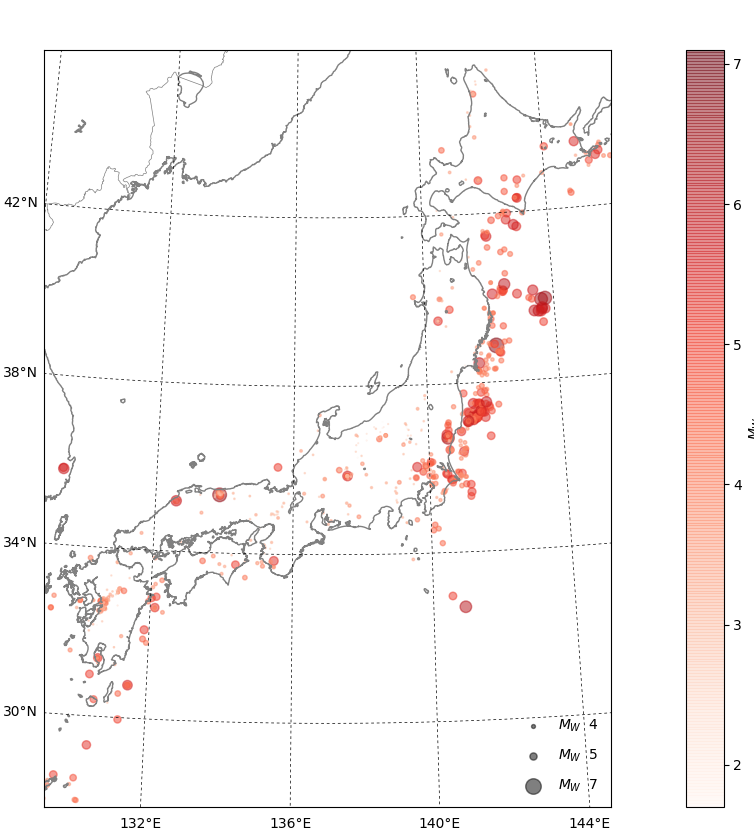
\includegraphics[width=0.8\linewidth]{img/basemap.jpg} 
 \renewcommand{\figurename}{图} 
\caption{全数据集地震事件} 
%英文标题begin 
\addtocounter{figure}{-1} \vspace{-5pt} 
%\SetEnglishCaption 
\renewcommand{\figurename}{Fig} 
\caption{Full data set earthquake event} 
\renewcommand{\figurename}{图} 
%英文标题end 
\label{fig:network-device-influence.png} 
\end{figure}
\indent 图5(a)显示了不同震级的地震数目分布。总体来看震级分布十分不均匀,小地震远多于大地震。但大地震破坏力大危害深重是我们在紧急预警系统中容错率低的部分,其在原始分布中、在训练集中出现频率低,不利于模型学习到关于如何预估大型地震震级的规则,给模型的训练带来较大的困扰。我们采取在训练集中对大地震数据过采样再加一定噪音的方法,以此处理数据分布不平衡问题。将原始的如图5(a)分布修正为图5(b),一定程度上缓解该问题。\\
\begin{figure}[!h] 
\centering 
 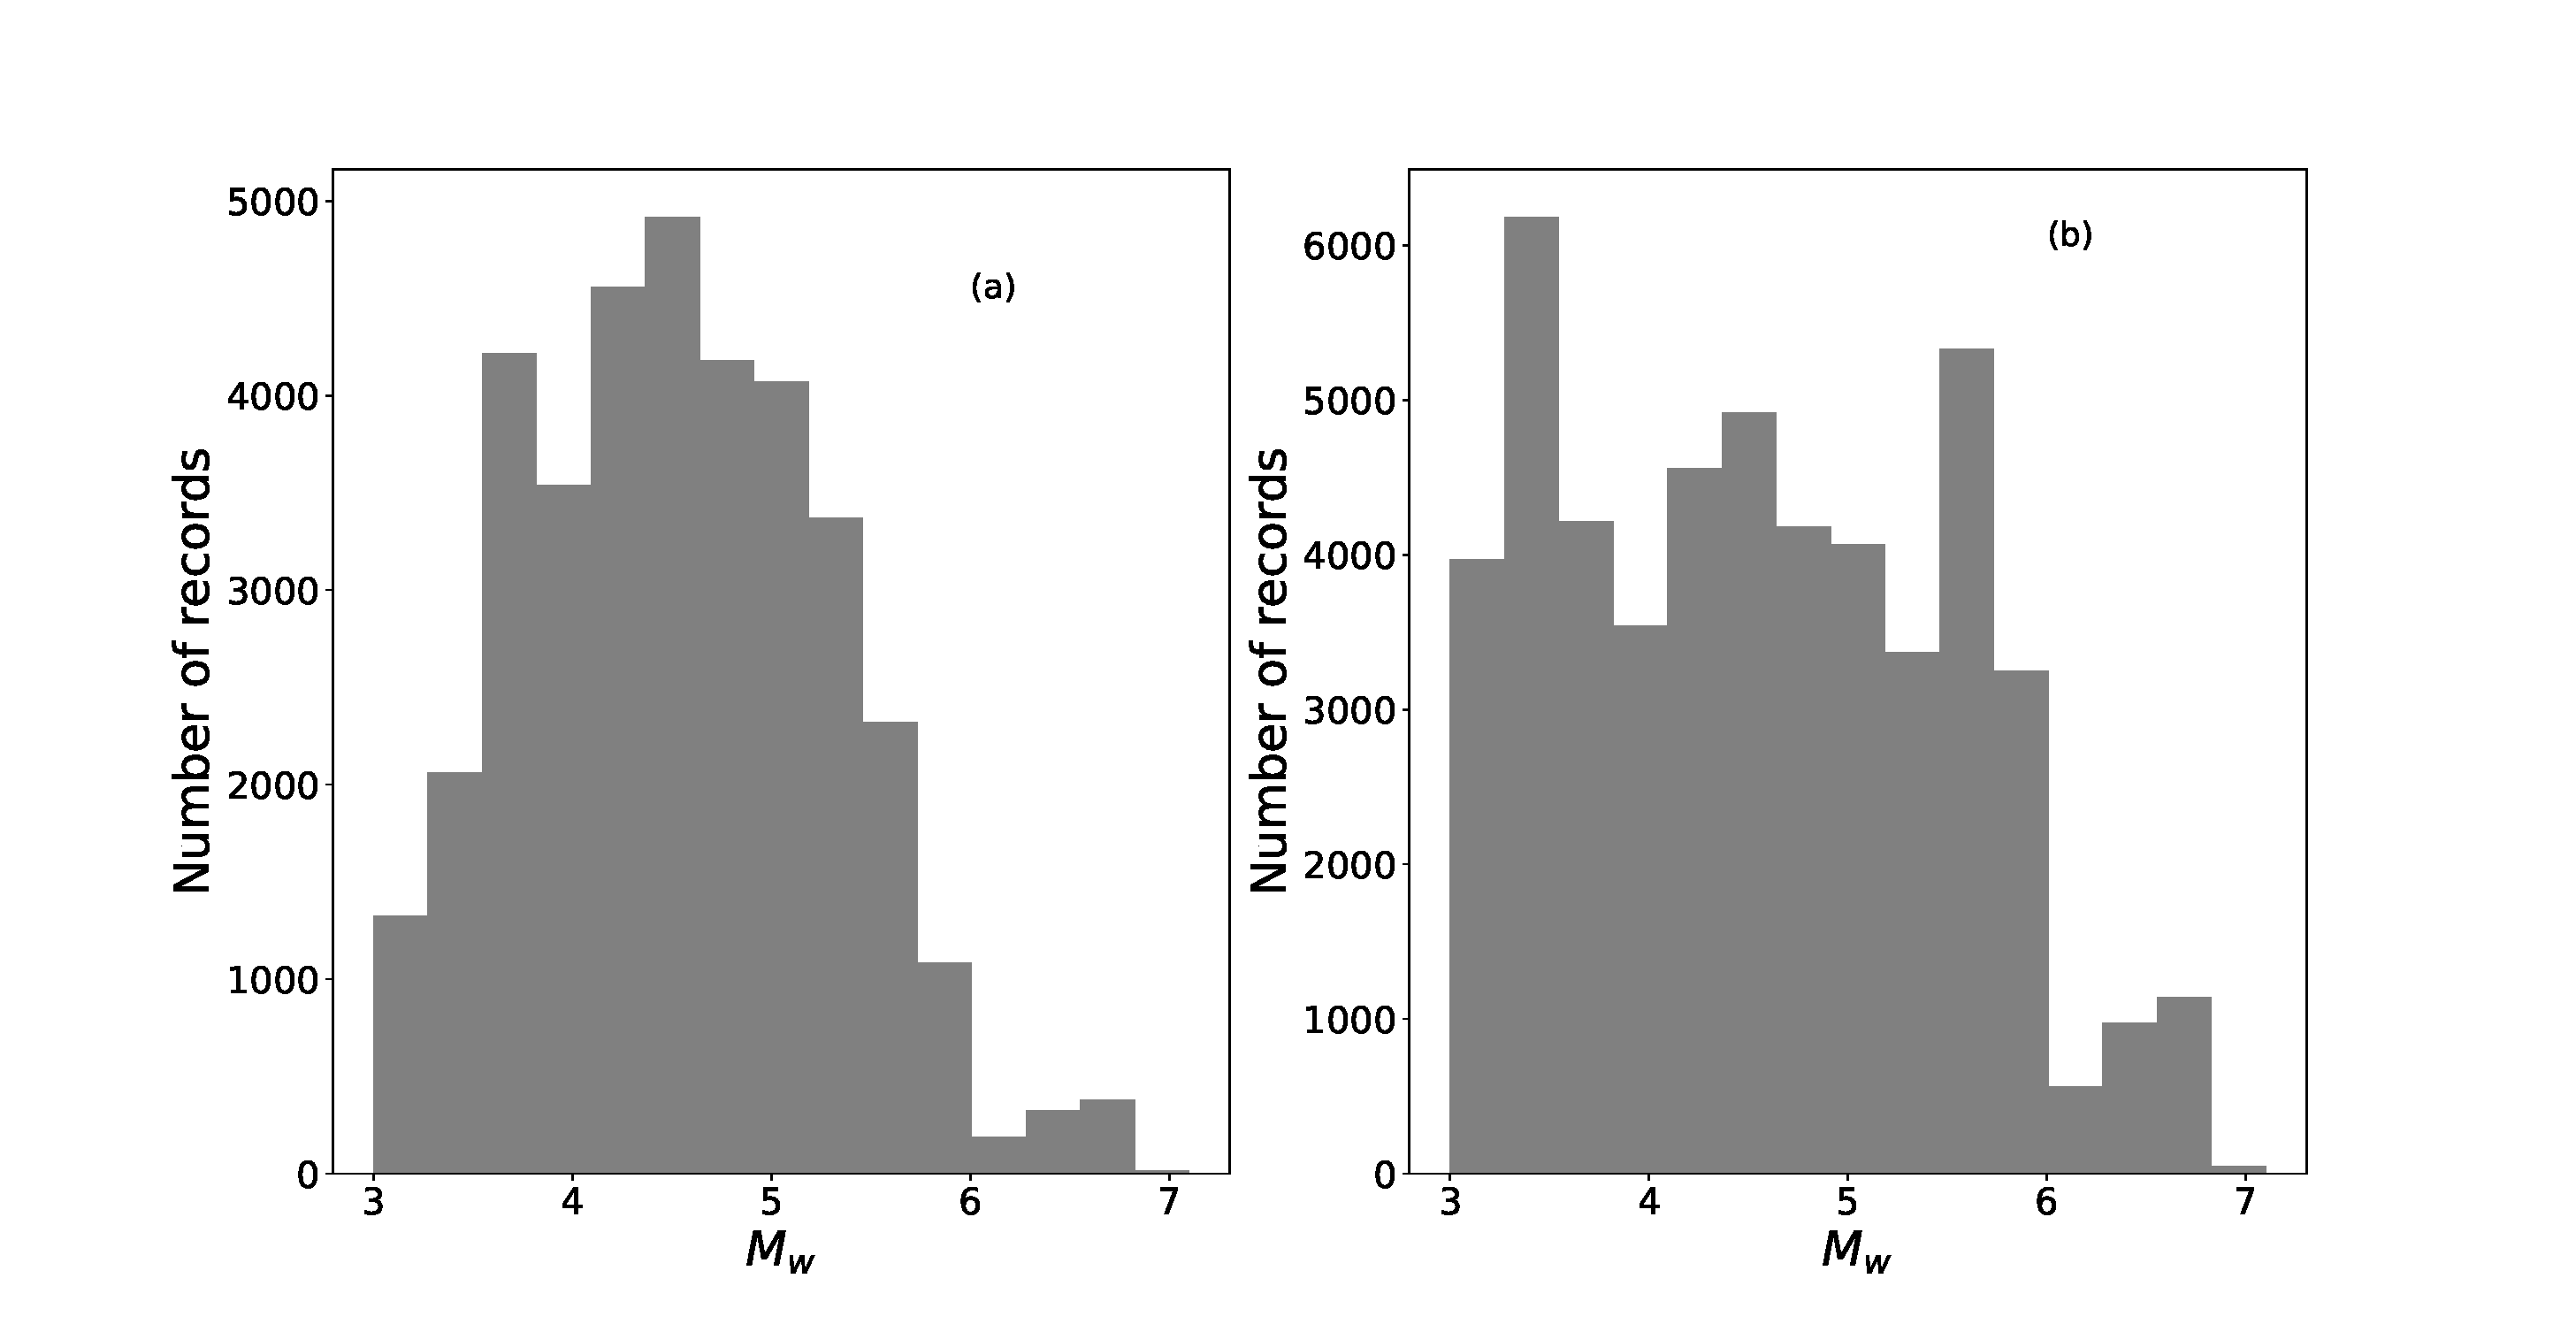
\includegraphics[width=0.8\linewidth]{img/5event_distribution.eps} 
 \renewcommand{\figurename}{图} 
\caption{数据集中地震记录的震级分布。横轴为震级$\mathbf{M}_{\mathbf{w}}$,纵轴为该震级的台站记录数目。\\
(a) 原始分布;(b) 调整后分布} 
%英文标题begin 
\addtocounter{figure}{-1} \vspace{-5pt} 
%\SetEnglishCaption 
\renewcommand{\figurename}{Fig} 
\caption{Magnitude distribution of seismic records in data sets, The horizontal axis is the magnitude $\mathbf{M}_{\mathbf{w}}$, and the vertical axis is the number of stations recorded for this magnitude.\\
(a) Original distribution; (b) Adjusted distribution
} 
\renewcommand{\figurename}{图} 
%英文标题end 
\label{fig:network-device-influence.png} 
\end{figure}